\documentclass{article}

\usepackage{url}
\usepackage[hmargin=1.5in]{geometry}
\usepackage{amsmath}
\usepackage{amssymb}
%%\usepackage{amsthm}
\usepackage{graphicx}

%%\theoremstyle{definition}
%%\newtheorem{defn}{Definition}
%%\theoremstyle{plain}
%%\newtheorem{prop}{Proposition}

% convenience aliases
\newcommand{\maps}{\colon}

% symbology
\newcommand{\Z}{\mathbb{Z}}
\newcommand{\R}{\mathbb{R}}
\newcommand{\C}{\mathbb{C}}
\newcommand{\laplace}{\mathcal{L}}
\DeclareMathOperator{\Ai}{Ai}

\title{Resurgence of the Airy function}
\author{Aaron Fenyes}

\begin{document}
\maketitle
\section{The Laplace transform}
\subsection{Analytic version}
\subsubsection{Regularity and decay properties}\label{reg-decay}
Take two copies $\R$ and $\hat{\R}$ of the real line, with standard coordinates $z$ and $\zeta$ respectively. The Laplace transform in $\zeta$ turns a function $\hat{\varphi}$ on $\hat{\R}_{\zeta > 0}$ into a function $\laplace_\zeta \hat{\varphi}$ on $\R_{z > 0}$, defined by the integral
\[ \laplace_\zeta \hat{\varphi} = \int_0^\infty e^{-z \zeta}\,\hat{\varphi}\;d\zeta. \]
For $a \in [0, \infty]$, recall that recall that $O_{\zeta \to a}(g)$ is the space of functions $\varphi$ on $\hat{\R}_{\zeta > 0}$ with $|\varphi| \lesssim g$ in some neighborhood of $a$. A function is {\em subexponential} if it's in $O_{\zeta \to \infty}(e^{c\zeta})$ for all $c > 0$. Let $\mathcal{E}_\zeta$ be the space of subexponential functions on $\hat{\R}_{\zeta > 0}$ which are $L^1$ both locally and around $\zeta = 0$. If $\hat{\varphi}$ is in $\mathcal{E}_\zeta$, then $\varphi = \laplace_\zeta \hat{\varphi}$ is well-defined, and it extends to a holomorphic function on the right half-plane $\C_{\operatorname{Re}(z) > 0}$~\cite[\S 5.6]{diverg-resurg-i}. If $\hat{\varphi}$ is in $O_{\zeta \to 0}(1)$, then $\varphi$ is in $O_{z \to \infty}(z^{-1})$~\cite[equation~1.8]{laplace-tfm}.\footnote{The argument cited still works in our generality. For holomorphic $\hat{\varphi}$, one can also use Equation 1.5 of {\em Borel-Laplace Transform and Asymptotic Theory} \textbf{(Sternin \& Shatalov)}.} More generally, if $\hat{\varphi}$ is in $O_{\zeta \to 0}(\zeta^{\alpha})$, with $\alpha > -1$, then $\varphi$ is in $O_{z \to \infty}\big(z^{-(\alpha + 1)}\big)$.
\subsubsection{Action on differential operators}\label{L-diff-op}
When $\hat{\varphi} \in \mathcal{E}_\zeta$, we can use differentiation under the integral to show that~\cite[Theorem~1.34]{laplace-tfm}
\begin{equation}\label{id:L-mult}
\laplace_\zeta (\zeta^n \hat{\varphi}) = \big({-\tfrac{\partial}{\partial z}}\big)^n \laplace_\zeta \hat{\varphi}.
\end{equation}

When $\hat{\varphi}$ is $n$ times differentiable, its $n$th derivative is in $\mathcal{E}$, and its zeroth through $(n - 1)$st derivatives extend continuously to zero, integration by parts gives the formula
\begin{align}\label{id:L-diff}
\laplace_\zeta \big(\tfrac{\partial}{\partial \zeta}\big)^n \hat{\varphi} & = z^n \laplace_\zeta \hat{\varphi} - \left[ \hat{\varphi}\,z^{n-1} + \hat{\varphi}'\,z^{n-2} + \hat{\varphi}''\,z^{n-3} + \ldots + \hat{\varphi}^{(n-1)} \right]_{\zeta = 0} \\
& = z^n\,\laplace\left( \hat{\varphi} - \left[ \hat{\varphi} + \hat{\varphi}'\,\zeta + \tfrac{\hat{\varphi}''}{2!}\,\zeta^2 + \ldots + \tfrac{\hat{\varphi}^{(n-1)}}{(n-1)!}\,\zeta^{n-1} \right]_{\zeta = 0} \right). \nonumber
\end{align}
Note that if a function's derivative is subexponential, so is the function itself.\footnote{Say $f' \in O_{\zeta \to \infty}(e^{c\zeta})$. Then \[ \left|\int_0^Z f'\,d\zeta\right| \le \int_0^Z |f'|\,d\zeta \lesssim \int_0^Z e^{c\zeta}\,d\zeta = \tfrac{1}{c}(e^{cZ} - 1) \lesssim e^{cZ}.\] Now we know the integral on the left-hand side converges, implying that $f$ extends continuously to zero, with $|f - f_{\zeta = 0}| \lesssim e^{c\zeta}$.}

%%In the space of holomorphic functions on the right half-plane, $\C[z] + O(z^{-1})$ is a direct sum, so there's a unique linear projection $\Lambda \maps \C[z] + O(z^{-1}) \to O(z^{-1})$. Applying $\Lambda$ to both sides of the formula above reveals that
%%\[ \laplace \big(\tfrac{\partial}{\partial \zeta}\big)^n \hat{\varphi} = \Lambda (z^n\,\laplace \hat{\varphi}). \]

%%Say $A$ is an $n$th-order differential operator with polynomial coefficients. If we know that $A\hat{\varphi} = 0$, and we know the Taylor polynomial of $\hat{\varphi}$ at zero through degree $n - 1$, we can use the formulas above to find an inhomogeneous differential equation that $\laplace \hat{\varphi}$ must satisfy.
\subsection{Algebraic version}
\subsubsection{Definition}
Let $\mathcal{P}_\zeta$ be the vector space spanned by $\zeta^\alpha$ for $\alpha \in \R \smallsetminus \Z_{< 0}$. Note that $\mathcal{P}_\zeta \cap \mathcal{E}_\zeta$ is $\mathcal{P}_\zeta^{> -1}$, the subspace spanned by $\zeta^\alpha$ with $\alpha > -1$. Since
\[ \laplace_\zeta(\zeta^\alpha) = \Gamma(\alpha+1)\,z^{-(\alpha + 1)} \]
for all $\alpha > -1$, let's use the same formula to extend $\laplace_\zeta$ to all of $\mathcal{P}_\zeta$. This defines $\laplace_\zeta$ consistently on $\mathcal{E}_\zeta + \mathcal{P}_\zeta$.
\subsubsection{Action on differential operators}\label{L-diff-op-alg}
Observe that
\[ \laplace_\zeta(\zeta^{\alpha + 1}) = -\tfrac{\partial}{\partial z}\,\laplace_\zeta(\zeta^\alpha) \]
for $\alpha \neq -1$. This extends identity~\ref{id:L-mult} to all of $\mathcal{P}_\zeta$.

Observe that
\[ \laplace_\zeta\tfrac{\partial}{\partial \zeta}(\zeta^\alpha) = \begin{cases}
z\,\laplace_\zeta(\zeta^\alpha) & \alpha \neq 0 \\
0 & \alpha = 0,
\end{cases} \]
and that $0 = z\,\laplace_\zeta(1) - 1$. This recovers identity~\ref{id:L-diff} for any function in $\mathcal{P}_\zeta$ whose $n$th derivative is in $\mathcal{P}_\zeta^{> -1}$. Although the functions in $\mathcal{P}_\zeta^{< 0}$ are singular at zero, let's pretend they vanish at zero. With that convention, formula~\ref{id:L-diff} extends to all of $\mathcal{P}_\zeta$.

Now we have the results of Section~\ref{L-diff-op} for all functions in $\mathcal{E}_\zeta + \mathcal{P}_\zeta$. Identity~\ref{id:L-diff} is particularly simple when $\hat{\varphi}$ has a {\em fractional power singularity} at $\zeta = 0$. By this, I mean that $\hat{\varphi}$ can be written as $\hat{\varphi}_\text{frac} + \hat{\varphi}_\text{reg}$, where $\hat{\varphi}_\text{frac} \in \mathcal{P}_\zeta$ has only non-integer exponents, and the zeroth through $(n-1)$st derivatives of $\hat{\varphi}_\text{reg} \in \mathcal{E}_\zeta$ vanish at zero. Under this condition, all the initial value terms in the identity vanish, leaving
\[ \laplace_\zeta \big(\tfrac{\partial}{\partial \zeta}\big)^n \hat{\varphi} = z^n \laplace_\zeta \hat{\varphi}. \]
\subsection{Change of coordinates}
Define a new coordinate $\zeta_a$ on $\hat{\R}$ so that $\zeta = a + \zeta_a$. From the calculation
\begin{align*}
\laplace_\zeta \hat{\varphi} & = \int_0^\infty e^{-z \zeta}\,\hat{\varphi}\;d\zeta \\
& = \int_0^\infty e^{-z(a + \zeta_a)}\,\hat{\varphi}\;d\zeta_a \\
& = e^{-az} \int_0^\infty e^{-z\zeta_a}\,\hat{\varphi}\;d\zeta_a \\
& = e^{-az} \laplace_{\zeta_a} \hat{\varphi},
\end{align*}
we learn that
\[ \laplace_{\zeta_a} \hat{\varphi} = e^{az} \laplace_\zeta \hat{\varphi}. \]

Define new coordinates $x$ and $\xi$ on $\R$ and $\hat{\R}$, respectively, so that $\zeta = b\xi$ and $z\,d\zeta = x\,d\xi$. Explicitly, $z = b^{-1}x$. From the calculation
\begin{align*}
\laplace_\zeta \hat{\varphi} & = \int_0^\infty e^{-z \zeta}\,\hat{\varphi}\;d\zeta \\
& = \int_0^\infty e^{-x\xi}\,\hat{\varphi}\;b\,d\xi \\
& = b \laplace_\xi \hat{\varphi},
\end{align*}
we learn that
\[ \laplace_\xi \hat{\varphi} = b^{-1} \laplace_\zeta \hat{\varphi}. \]
\section{The Airy equation}
\subsection{Basics}
The Airy equation is
\begin{equation}\label{eqn:airy}
\left[\big(\tfrac{\partial}{\partial y}\big)^2 - y\right] \psi = 0.
\end{equation}
One solution is given by the Airy function,
\[ \Ai(y) = \frac{i}{2\pi} \int_{\Gamma} \exp\left(-\tfrac{1}{3}t^3 + yt\right)\,dt, \]
where $\Gamma$ is a path that comes from $\infty$ at $120^\circ$ and goes to $\infty$ at $-120^\circ$.
\begin{center}
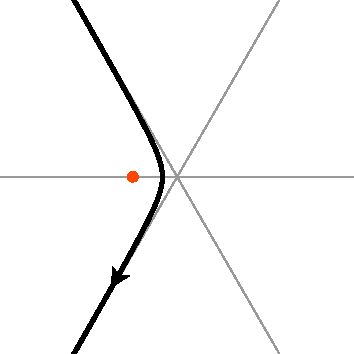
\includegraphics{figures/u_contour.pdf} \\[1em]
{\small The contour $\Gamma$ in the $u$ plane.}
\end{center}
With the substitution $t = 2uy^{1/2}$, we can rewrite the Airy integral as
\[ \Ai(y) = y^{1/2}\;\frac{i}{\pi} \int_{y^{-1/2} \Gamma} \exp\left[-\tfrac{2}{3}y^{3/2} \left(4u^3 - 3u\right)\right]\,du. \]
We've rescaled the contour by a factor of two, but it still approaches $\infty$ in the desired way. Note that $4u^3 - 3u$ is the third Chebyshev polynomial.
\subsection{Rewriting as a modified Bessel equation}
We can distill the most interesting part of the Airy function by writing
\[ \Ai(y) = \tfrac{1}{\pi\sqrt{3}}\,y^{1/2}\, K\big(\tfrac{2}{3} y^{3/2}\big), \]
where
\begin{equation}\label{integral:mod-bessel}
K(z) = i\sqrt{3} \int_{z^{-1/3}\Gamma} \exp\left[-z \left(4u^3 - 3u\right)\right]\,du.
\end{equation}
Saying that $\Ai$ satisfies the Airy equation is equivalent to saying that $K$ satisfies the modified Bessel equation
\begin{equation}\label{eqn:mod-bessel}
\left[z^2 \big(\tfrac{\partial}{\partial z}\big)^2 + z \tfrac{\partial}{\partial z} - \big[\big(\tfrac{1}{3}\big)^2 + z^2\big]\right] \varphi = 0.
\end{equation}
In fact, $K$ is the modified Bessel function $K_{1/3}$~\cite[equation~9.6.1]{dlmf}.

As we'll see in Section~\ref{asymp}, $K$ is in $O_{z \to \infty}(e^{-z})$. It'll be helpful to pull out the exponential decay factor and work instead with the function $\kappa$ defined by $K = e^{-z} \kappa$. Saying that $K$ satisfies equation~\ref{eqn:mod-bessel} is equivalent to saying that $\kappa$ satisfies the equation
\begin{equation}\label{eqn:shifted-mod-bessel}
\left[z^2 \big(\tfrac{\partial}{\partial z} + 1\big)^2 + z \big(\tfrac{\partial}{\partial z} + 1\big) - \big[\big(\tfrac{1}{3}\big)^2 + z^2\big]\right] \varphi = 0.
\end{equation}
\subsection{Asymptotic analysis}
From \cite{dlmf}, equations 10.40.2 and 10.17.1, we get the asymptotic series
\begin{equation}\label{bessel-asymp}
\kappa \sim \left(\tfrac{\pi}{2}\right)^{1/2} \left[ z^{-1/2} - \frac{(\tfrac{1}{6})_1 (\tfrac{5}{6})_1}{2^1 \cdot 1!}\;z^{-3/2} + \frac{(\tfrac{1}{6})_2 (\tfrac{5}{6})_2}{2^2 \cdot 2!}\;z^{-5/2} - \frac{(\tfrac{1}{6})_3 (\tfrac{5}{6})_3}{2^3 \cdot 3!}\;z^{-7/2} + \ldots \right]
\end{equation}
\subsection{Going to the spatial domain}\label{spatial}
\subsubsection{A good try at $\zeta = 0$}
Let's try to find a function $\hat{K}$ with $K = \laplace_\zeta \hat{K}$, which is unique if it exists~\cite[Theorem~1.23]{laplace-tfm}. If a function $\hat{\varphi}$ satisfies the equation
\begin{equation}\label{eqn:spatial-mod-bessel}
\left[\big(\zeta^2 - 1\big) \big(\tfrac{\partial}{\partial \zeta}\big)^2 + 3\zeta \tfrac{\partial}{\partial \zeta} + \big[1 - \big(\tfrac{1}{3}\big)^2\big]\right] \hat{\varphi} = 0,
\end{equation}
its Laplace transform $\varphi = \laplace_\zeta \hat{\varphi}$ satisfies the equation
\begin{align*}
\left[\big({-\tfrac{\partial}{\partial z}}\big)^2 - 1\right] \Big(z^2 \varphi - \big[\hat{\varphi}\,z + \hat{\varphi}'\big]_{\zeta = 0}\Big) + 3\big({-\tfrac{\partial}{\partial z}}\big)\big[z\varphi - \hat{\varphi}\big]_{\zeta = 0} + \big[1 - \big(\tfrac{1}{3}\big)^2\big] \varphi & = 0 \\
\big(\tfrac{\partial}{\partial z}\big)^2 \big[z^2 \varphi\big] - \Big(z^2 \varphi - \big[\hat{\varphi}\,z + \hat{\varphi}'\big]_{\zeta = 0}\Big) - 3\big(\tfrac{\partial}{\partial z}\big)\big[z\varphi\big] + \big[1 - \big(\tfrac{1}{3}\big)^2\big] \varphi & = 0 \\
\Big[2 + 4z\tfrac{\partial}{\partial z} + z^2\big(\tfrac{\partial}{\partial z}\big)^2\Big]\varphi - \Big(z^2 \varphi - \big[\hat{\varphi}\,z + \hat{\varphi}'\big]_{\zeta = 0}\Big) - 3\Big[1 + z\tfrac{\partial}{\partial z}\Big]\varphi + \big[1 - \big(\tfrac{1}{3}\big)^2\big] \varphi & = 0,
\end{align*}
which simplifies to
\begin{equation}\label{eqn:inhomog-mod-bessel}
\left[z^2 \big(\tfrac{\partial}{\partial z}\big)^2 + z \tfrac{\partial}{\partial z} - \big[\big(\tfrac{1}{3}\big)^2 + z^2\big]\right] \varphi = -\big[\hat{\varphi}\,z + \hat{\varphi}'\big]_{\zeta = 0}.
\end{equation}
Since we want $\laplace_\zeta \hat{K}$ to satisfy equation~\ref{eqn:mod-bessel}, which is the homogeneous version of equation~\ref{eqn:inhomog-mod-bessel}, we might guess that $\hat{K}$ is a solution of equation~\ref{eqn:spatial-mod-bessel} that vanishes through first order at $\zeta = 0$. Unfortunately, this would force $\hat{K}$ to be zero.
\subsubsection{Success at $\zeta = 1$}\label{spatial-success}
Define a new coordinate $\zeta_1$ on $\hat{\R}$ so that $\zeta = 1 + \zeta_1$. Since
\begin{align*}
\laplace_{\zeta_1} \hat{K} & = e^z \laplace_\zeta \hat{K} \\
& = e^z K \\
& = \kappa,
\end{align*}
we want $\laplace_{\zeta_1} \hat{K}$ to satisfy equation~\ref{eqn:shifted-mod-bessel}. Rewrite equation~\ref{eqn:spatial-mod-bessel} as
\begin{equation}\label{eqn:shifted-spatial-mod-bessel}
\left[\zeta_1(\zeta_1 + 2) \big(\tfrac{\partial}{\partial \zeta_1}\big)^2 + 3(\zeta_1 + 1) \tfrac{\partial}{\partial \zeta_1} + \big[1 - \big(\tfrac{1}{3}\big)^2\big]\right] \hat{\varphi} = 0.
\end{equation}
If $\hat{\varphi}$ satisfies equation~\ref{eqn:shifted-spatial-mod-bessel}, $\laplace_{\zeta_1} \hat{\varphi}$ will satisfy an inhomogeneous version of equation~\ref{eqn:shifted-mod-bessel}, analogous to equation~\ref{eqn:inhomog-mod-bessel}. This time, though, there's a trick we can use to zero out the inhomogeneity. Equation~\ref{eqn:shifted-spatial-mod-bessel} has a regular singularity at $\zeta_1 = 0$, and one solution (up to scaling) is a holomorphic multiple of $\zeta_1^{-1/2}$. That solution has a fractional power singularity at $\zeta_1 = 0$, as defined in Section~\ref{L-diff-op-alg}, so its Laplace transform in $\zeta_1$ satisfies equation~\ref{eqn:shifted-mod-bessel}.

Following this plan, let's find $\hat{K}$ explicitly. Defining another coordinate $\xi$ on $\hat{\R}$ so that $\zeta_1 = -2\xi$, we can rewrite equation~\ref{eqn:shifted-spatial-mod-bessel} as the hypergeometric equation
\begin{equation}\label{eqn:hypergeom}
\left[\xi(1 - \xi) \big(\tfrac{\partial}{\partial \xi}\big)^2 + 3(\tfrac{1}{2} - \xi) \tfrac{\partial}{\partial \xi} - \big[1 - \big(\tfrac{1}{3}\big)^2\big]\right] \hat{\varphi} = 0.
\end{equation}
The hypergeometric function
\[ \hat{g}_1 = F\big(\tfrac{2}{3}, \tfrac{4}{3}; \tfrac{3}{2}; \xi\big) \]
satisfies equation~\ref{eqn:hypergeom} by definition. It's not the solution we want, though, because it's holomorphic around $\xi = 0$. Formula~15.10.12 from \cite{dlmf} gives another solution,
\[ \hat{f}_0 = \xi^{-1/2} F\big(\tfrac{1}{6}, \tfrac{5}{6}; \tfrac{1}{2}; \xi\big), \]
which is a holomorphic multiple of $\xi^{-1/2}$ near $\xi = 0$. By the argument above, $f_0 = \laplace_{\zeta_1} \hat{f}_0$ satisfies equation~\ref{eqn:shifted-mod-bessel}. This suggests that a constant multiple of $\hat{f}_0$ is our desired $\hat{K}$. The power series~\cite[equation~15.2.1]{dlmf}
\[ \hat{f}_0 = \xi^{-1/2} + \frac{(\tfrac{1}{6})_1 (\tfrac{5}{6})_1}{(\tfrac{1}{2})_1 \; 1!}\;\xi^{1/2} + \frac{(\tfrac{1}{6})_2 (\tfrac{5}{6})_2}{(\tfrac{1}{2})_2 \; 2!}\;\xi^{3/2} + \frac{(\tfrac{1}{6})_3 (\tfrac{5}{6})_3}{(\tfrac{1}{2})_3 \; 3!}\;\xi^{5/2} + \ldots \]
converges near $\xi = 0$, showing that
\[ \hat{f}_0 \in \xi^{-1/2} + O_{\xi \to 0}(\xi^{1/2}). \]
In terms of $\zeta_1$, we have
\[ \hat{f}_0 \in -i \sqrt{2}\,\zeta_1^{-1/2} + O_{\zeta_1 \to 0}(\zeta_1^{1/2}). \]
Using the decay properties from Section~\ref{reg-decay}, we deduce that
\[ f_0 \in -i \sqrt{2\pi}\,z^{-1/2} + O_{z \to \infty}(z^{-3/2}). \]
Since we know that $f_0$ satisfies equation~\ref{eqn:shifted-mod-bessel}, this confirms that $f_0$ is a constant multiple of $\kappa$, which is the only subexponential solution of equation~\ref{eqn:shifted-mod-bessel} (up to scaling). Comparing with series~\ref{bessel-asymp}, we see that $\kappa = i\,\tfrac{1}{2}\,f_0$. We conclude that $\kappa = \laplace_{\zeta_1} \hat{K}$ for
\[ \hat{K} = \tfrac{1}{\sqrt{2}}\,\zeta_1^{-1/2} F\big(\tfrac{1}{6}, \tfrac{5}{6}; \tfrac{1}{2}; -\tfrac{1}{2}\zeta_1\big). \]
\section{Sketches}
\subsection{Contour argument}
We can recast integral~\ref{integral:mod-bessel} into $\hat{\C}$ by setting $\zeta = 4u^3 - 3u$. Projecting $z^{-1/3} \Gamma$ to a contour $\gamma_z$ in $\hat{\C}$ and choosing the branch of $u$ that lifts $\gamma_z$ back to $z^{-1/3} \Gamma$, we have
\begin{equation}\label{integral:mod-bessel-zeta}
K(z) = \frac{i}{\sqrt{3}} \int_{\gamma_z} e^{-z\zeta}\frac{d\zeta}{4u^2 - 1}.
\end{equation}
For $z \in (0, \infty)$, the contour $\gamma(z)$ runs clockwise around $[1, \infty)$, as shown below. Let's assume $z \in (0, \infty)$ for the rest of the section. \textbf{[Our conclusions should probably hold whenever $\operatorname{Re}(z) > 0$.]}
\begin{center}
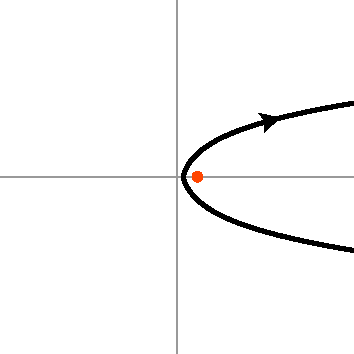
\includegraphics{figures/zeta_contour.pdf} \\[1em]
{\small The contour $\gamma_1$ in $\hat{\C}$.}
\end{center}

It happens\footnote{How to verify this? This hypergeometric function can be written in terms of Legendre functions, but I don't know where to go from there. \textbf{Veronica:} Look at ``Special cases'' section in \cite{dlmf}, e.g. 15.4.14!} that for our desired branch of $u$,
\[ \frac{1}{4u^2 - 1} = -F\big(\tfrac{1}{3}, \tfrac{2}{3}; \tfrac{1}{2}; \zeta^2\big), \]
so we can rewrite integral~\ref{integral:mod-bessel-zeta} as
\[ K(z) = \frac{1}{i\sqrt{3}} \int_{\gamma_z} e^{-z\zeta} F\big(\tfrac{1}{3}, \tfrac{2}{3}; \tfrac{1}{2}; \zeta^2\big)\;d\zeta. \]
This gives us an alternate route to the conclusion of Section~\ref{spatial}, which we'll follow below.

In addition to the solutions $\hat{g}_1$ and $\hat{f}_0$ from Section~\ref{spatial-success}, equation~\ref{eqn:hypergeom} has the solutions
\begin{alignat*}{2}
\hat{g}_0 &\;=\;& & F\big(\tfrac{2}{3}, \tfrac{4}{3}; \tfrac{3}{2}; 1-\xi\big) \\
\hat{f}_1 &\;=\;& (1-\xi)^{-1/2} & F\big(\tfrac{1}{6}, \tfrac{5}{6}; \tfrac{1}{2}; 1-\xi\big),
\end{alignat*}
given by formulas 15.10.13 and 15.10.14 from \cite{dlmf}. These four solutions are related by identities 15.10.18, and 15.10.22 from \cite{dlmf}:
\begin{alignat*}{3}
\hat{f}_1 &\;=\;&\tfrac{1}{\sqrt{3}}\,\hat{g}_1 &\;+\;& \tfrac{1}{2}\,\hat{f}_0 \\
\hat{f}_0 &\;=\;& \tfrac{1}{\sqrt{3}}\,\hat{g}_0 &\;+\;& \tfrac{1}{2}\,\hat{f}_1.
\end{alignat*}
Summing these identities, we see that
\[ \hat{g}_1 + \hat{g}_0 = \tfrac{\sqrt{3}}{2}\,(\hat{f}_1 + \hat{f}_0). \]

The quadratic transformation identity 15.8.27 from \cite{dlmf} shows \textbf{[verified numerically]} that\footnote{Note that $2\Gamma(\tfrac{1}{2})\Gamma(\tfrac{3}{2}) = 2\Gamma(\tfrac{1}{2})\,\tfrac{1}{2}\Gamma(\tfrac{1}{2}) = \pi$ and $\big[\Gamma(\tfrac{5}{6})\Gamma(\tfrac{7}{6})\big]^{-1} = \big[\Gamma(\tfrac{5}{6})\,\tfrac{1}{6}\Gamma(\tfrac{1}{6})\big]^{-1} = \frac{6\sin(\tfrac{1}{6} \pi)}{\pi} = \frac{3}{\pi}$.}
\begin{align*}
F\big(\tfrac{1}{3}, \tfrac{2}{3}; \tfrac{1}{2}; \zeta^2\big) & = \tfrac{1}{3}(\hat{g}_1 + \hat{g}_0) \\
& = \tfrac{1}{2\sqrt{3}}(\hat{f}_1 + \hat{f}_0)
\end{align*}
so we have
\[ K(z) = \frac{1}{6i} \int_{\gamma_z} e^{-z\zeta} (\hat{f}_1 + \hat{f}_0)\;d\zeta. \]
The solution $\hat{f}_1$ is regular on $\zeta \in [1, \infty)$, so it integrates to zero. \textbf{[This doesn't hold up numerically!]} The solution $\hat{f}_0$ looks like $(1 - \zeta)^{-1/2}$ times a function which is regular on $\zeta \in [1, \infty)$, so integrating it along $\gamma_z$ is the same as integrating it twice along the contour that goes rightward from $1$, with its value continued from above the singularity. Hence,
\begin{align*}
K(z) & = \frac{1}{3i} \int^\infty_1 e^{-z\zeta} \hat{f}_0\;d\zeta \\
& = \tfrac{1}{3i} \laplace_{\zeta_1} \hat{f}_0.
\end{align*}
\textbf{[Constant conflicts with Section~\ref{spatial}]}
\subsection{Correspondence with Mari\~{n}o's series}
Let $f_1(z)$ be the holomorphic function corresponding to Mari\~{n}o's formal power series $\varphi_1(z^{-1})$. The formal power series corresponding to $f$ will be written in the variable $z$.

\begin{align*}
\Ai(x) & = \tfrac{1}{2\sqrt{\pi}} x^{-1/4} e^{-z} \varphi_1\big(\tfrac{2}{3} z^{-1}\big) \\
& = \tfrac{1}{2\sqrt{\pi}} x^{-1/4} e^{-z} f_1\big(\tfrac{3}{2} z\big) \\
\Ai(x) & = \frac{1}{\pi\sqrt{3}} x^{1/2} K(\tfrac{2}{3} x^{3/2})
\end{align*}
Putting together,
\begin{align*}
\tfrac{1}{2\sqrt{\pi}} x^{-1/4} e^{-z} f_1\big(\tfrac{3}{2} z\big) & = \frac{1}{\pi\sqrt{3}} x^{1/2} K(\tfrac{2}{3} x^{3/2}) \\
\tfrac{\sqrt{3\pi}}{2}\;x^{-3/4} e^{-z} f_1\big(\tfrac{3}{2} z\big) & = K(\tfrac{2}{3} x^{3/2}) \\
\tfrac{\sqrt{3\pi}}{2}\;\big(\tfrac{3}{2} z)^{-1/2} e^{-z} f_1\big(\tfrac{3}{2} z\big) & = K(z) \\
\sqrt{\tfrac{\pi}{2}}\;z^{-1/2} e^{-z} f_1\big(\tfrac{3}{2} z\big) & = K(z) \\
\sqrt{\tfrac{\pi}{2}}\;\big[\laplace^{-1} z^{-1/2}\big] * \big[\laplace^{-1} f_1\big(\tfrac{3}{2} z\big)\big](\zeta - 1) & = \hat{K}(\zeta) \\
\sqrt{\tfrac{\pi}{2}}\;\left[\Gamma\big({-\tfrac{1}{2}}\big)^{-1} \zeta^{-1/2}\right] * \tfrac{2}{3} \hat{f}_1\big[\tfrac{2}{3}(\zeta - 1)\big] & = \hat{K}(\zeta) \\
-\tfrac{1}{3\sqrt{2}}\;\left[\zeta^{-1/2}\right] * \hat{f}_1\big[\tfrac{2}{3}(\zeta - 1)\big] & = \hat{K}(\zeta) \\
\end{align*}
Notice that if the hypergeometric differentiation formula holds for fractional derivatives,
\[ \big(\tfrac{\partial}{\partial \xi}\big)^{1/2}F\big(\tfrac{2}{3}, \tfrac{4}{3}; \tfrac{3}{2}; \xi\big) \propto F\big(\tfrac{7}{6}, \tfrac{11}{6}; 2; \xi\big) \]
\bibliographystyle{utphys}
\bibliography{airy-resurgence}
\end{document}